\section{Pregunta 1: Salto del cuadrúpedo sobre un obstáculo}
\label{sec:p1}

\subsection{Descripción del problema}
El cuadrúpedo parte en reposo con el CdM en $\bp_0=(0,0,0.30)$\,m y termina en reposo en $\bp_f=(1.20,0,0.30)$\,m. Entre ambos puntos hay una caja de altura $H=0.25$\,m que ocupa $x\in[x_1,x_2]=[0.42,0.67]$\,m y todo el ancho del robot. Todos los parámetros se leen del URDF del robot mediante el módulo \texttt{go2\_modelo.py}. El marco del cuerpo $\{B\}$ tiene $x$ hacia adelante, $y$ hacia la izquierda y $z$ hacia arriba; las patas se ordenan FR, FL, RR, RL.

\subsection{Modelo dinámico: SRBM}
Se usa el SRBM con patas sin masa. El estado y la entrada son
\begin{align*}
    \bx&=\begin{bmatrix}\bp\tr&\bm{\eta}\tr&\bv\tr&{}^b\bomega\tr\end{bmatrix}\tr\!\in\RR^{12},\\
    \bu&=\begin{bmatrix}\bef_{FR}\tr&\bef_{FL}\tr&\bef_{RR}\tr&\bef_{RL}\tr\end{bmatrix}\tr\!\in\RR^{12},
\end{align*}
donde $\bm{\eta}=(\phi,\theta,\psi)$ son los ángulos roll--pitch--yaw y $\bef_i$ es la fuerza del suelo sobre el pie $i$, ubicado en $\bp_i$. La dinámica es
\begin{align*}
\dot{\bp}&=\bv, \\
\dot{\bv}&=\mathbf{g}+\tfrac{1}{m}\textstyle\sum_{i=1}^{4}\bef_i,\\
\dot{\bm{\eta}}&=E(\phi,\theta)\,{}^b\bomega,\\
I\,{}^b\dot{\bomega}&={}^w\bR_b\tr\!\sum_{i=1}^{4}(\bp_i-\bp)\times\bef_i-{}^b\bomega\times(I\,{}^b\bomega),
\end{align*}
con $\mathbf{g}=(0,0,-g)\tr$, $\bR={}^w\bR_b=\bR_z(\psi)\bR_y(\theta)\bR_x(\phi)$ y

\begin{equation*}
E(\phi,\theta)=\begin{bmatrix}
1&\sin\phi\tan\theta&\cos\phi\tan\theta\\
0&\cos\phi&-\sin\phi\\
0&\sin\phi/\cos\theta&\cos\phi/\cos\theta
\end{bmatrix}.
\end{equation*}

\textbf{Integrador.} Cada intervalo $[t_k,t_{k+1}]$ de duración $h_k$ se integra con RK4 en dos subpasos de $h_k/2$, con fuerzas constantes en el intervalo:
\begin{equation*}
\hat{\bx}_{k+1}=\bm{\Psi}_k(\bx_k,\bu_k,h_k)\equiv\Phi^{\mathrm{RK4}}\!\left(\bx_k,\bu_k,\bp^c_k,h_k\right),
\end{equation*}
donde $\bp^c_k\in\RR^{12}$ agrupa las posiciones de los cuatro pies en $\{W\}$ durante el intervalo $k$.

\subsection{Secuencia de contactos}
El salto se divide en cinco fases $j=1,\dots,5$ con conjunto de patas en apoyo $\mathcal S_j$ (Tabla~\ref{tab:fases}). El número de intervalos $N_j$ es fijo; la duración $T_j$ de cada fase es variable de decisión acotada.

\begin{table}[h]
\caption{Secuencia de contactos del salto.}
\label{tab:fases}
\centering
\begin{tabular}{@{}clcccc@{}}
\toprule
$j$ & Descripción & $\mathcal S_j$ & $N_j$ & $T_j^{\min}$ & $T_j^{\max}$ \\
\midrule
1 & Impulso con 4 patas & FR, FL, RR, RL & 22 & 0.25 & 0.80\\
2 & Impulso con traseras & RR, RL & 10 & 0.05 & 0.15\\
3 & Vuelo & $\emptyset$ & 24 & 0.15 & 1.70\\
4 & Aterrizaje delanteras & FR, FL & 10 & 0.05 & 0.15\\
5 & Apoyo con 4 patas & FR, FL, RR, RL & 22 & 0.25 & 0.80\\
\bottomrule
\end{tabular}
\end{table}

Las fases se concatenan en una sola malla de
\begin{equation*}
N=\sum_{j=1}^{5}N_j=22+10+24+10+22=88
\end{equation*}
intervalos, con $h_k=T_{j(k)}/N_{j(k)}$ y $t_{k+1}=t_k+h_k$, donde $j(k)$ es la fase del intervalo $k$. Los pies en contacto antes del despegue permanecen fijos en $\bp^{c}_i=(x^{0}_i,y_i,0)$; los pies que aterrizan se ubican en $(x^a_i,y_i,0)$, con $x^a_i$ variable de decisión.

\subsection{Restricciones}
\subsubsection{Fuerzas de contacto}
Para cada pata $i\in\mathcal S_{j(k)}$ se impone unilateralidad, fuerza normal máxima y pirámide de fricción con $\mu=0.7$ y $f_{\max}=220$\,N:
\begin{equation*}
0\le f_{z,i}\le f_{\max},\quad |f_{x,i}|\le\mu f_{z,i},\quad |f_{y,i}|\le\mu f_{z,i}.
\end{equation*}
Si $i\notin\mathcal S_{j(k)}$ (pie en el aire): $\bef_{i,k}=\mathbf 0$.

\subsubsection{Alcance cinemático de las patas}
Para las patas en apoyo, con $\bd_i={}^w\bR_b\tr(\bp^c_i-\bp)-\mathbf r^{cad}_i$ el vector cadera--pie en $\{B\}$:
\begin{equation*}
0.20\le\|\bd_i\|\le0.39,\qquad |d_{i,x}|\le0.20 .
\end{equation*}

\subsubsection{Obstáculo suave}
Para que la restricción sea diferenciable, la caja se aproxima con el producto de dos sigmoides, inflado por un margen $\delta=3$\,cm:
\begin{equation*}
h_{\mathrm{obs}}(x)=(H+\delta)\,\sigma\!\big(k(x-x_1+\delta)\big)\,\sigma\!\big(k(x_2+\delta-x)\big),
\end{equation*}
con $\sigma(s)=1/(1+e^{-s})$ y $k=80$. Cada punto $c=(x_c,y_c,z_c)$ relevante del robot debe cumplir $z_c\ge h_{\mathrm{obs}}(x_c)$. Los puntos considerados son: las cuatro esquinas inferiores del tronco, el pie y la rodilla de las patas recogidas en el aire, y la rodilla de las patas en apoyo.

\subsubsection{Ventanas de extensión de las patas}
Las patas recogidas en vuelo ($\mathrm{pie}_z=-0.12$\,m en $\{B\}$, pose $(q_1^{rec},q_2^{rec})$) deben extenderse para aterrizar.
Para evitar colisiones durante la extensión, en las ventanas indicadas se exige que rodilla y pie, a lo largo de la interpolación $(1-s_b)\,\bm q^{rec}+s_b\,\bm q^{td}$, $s_b\in\{0.25,0.5,0.75,1\}$, cumplan $z_c\ge h_{\mathrm{obs}}(x_c)$, donde $\bm q^{td}$ es la configuración al instante de contacto.

\subsubsection{Orientación y duraciones}
Se imponen $|\phi|\le0.3$\,rad, $|\theta|\le0.8$\,rad y $T_j^{\min}\le T_j\le T_j^{\max}$. Los pies aterrizan después del obstáculo, $x^a_i\ge x_2+0.06$, en postura final nominal ($|x^a_i-(x_f+s_{x,i}\,h_x)|\le0.04$) y con simetría izquierda/derecha ($x^a_{FR}=x^a_{FL}$, $x^a_{RR}=x^a_{RL}$). Las restricciones geométricas y de orientación se evalúan en los nodos $\bx_k$ y en el punto medio $\bx_{k+1/2}=\bm\Psi_k(\bx_k,\bu_k,h_k/2)$ de cada intervalo.

\subsection{Formulación del NLP}
\textbf{Vector de decisión:}
\begin{equation*}
\bz=\big(\bx_1,\dots,\bx_N,\ \bu_0,\dots,\bu_{N-1},\ T_1,\dots,T_5,\ x^a_1,\dots,x^a_4\big),
\end{equation*}
con $\bx_0=\bx_{\mathrm{ini}}=(0,0,0.30,\mathbf 0)$ fijo.

\textbf{Costo:} 
\begin{equation*}
J(\bz)=\sum_{k=0}^{N-1}h_k\,\ell_k+0.02\sum_{k=1}^{N-1}\Big\|\tfrac{\bu_k-\bu_{k-1}}{mg}\Big\|^2,
\end{equation*}
\begin{equation*}
\ell_k=\Big\|\tfrac{\bu_k-\bu^{\mathrm{est}}_k}{mg}\Big\|^2+0.05\|{}^b\bomega_k\|^2+2(\phi_k^2+\psi_k^2),
\end{equation*}
donde $\bu^{\mathrm{est}}_k$ reparte el peso $mg$ en partes iguales entre las patas en apoyo (apoyo estático), de modo que se penaliza la desviación respecto de éste.

\textbf{Problema discretizado:}
\begin{equation*}
\begin{aligned}
\min_{\bz}\quad & J(\bz)\\
\text{s.a.}\quad
& \bx_{k+1}-\bm\Psi_k(\bx_k,\bu_k,h_k)=\mathbf 0, && k=0,\dots,N-1\\
& \bx_N-\bx_f=\mathbf 0, && \bx_f=(1.20,0,0.30,\mathbf 0)\\
& \bef_{i,k}=\mathbf 0,\ \ i\notin\mathcal S_{j(k)}, && k=0,\dots,N-1\\
& \mathbf c_{\mathrm{ineq}}(\bx_k,\bx_{k+1/2},\bu_k)\le\mathbf 0, && k=0,\dots,N-1\\
& \bx_{\min}\le\bx_k\le\bx_{\max}, && k=1,\dots,N\\
& T_j^{\min}\le T_j\le T_j^{\max}, && j=1,\dots,5.
\end{aligned}
\end{equation*}

$\mathbf c_{\mathrm{ineq}}$ agrupa fricción, unilateralidad y $f_{\max}$, alcance de las patas, obstáculo y los pies de aterrizaje. Cada intervalo aporta $12$ igualdades de continuidad, de modo que hay $12N=1056$ restricciones dinámicas.

\textbf{Inicialización.} Se usa una trayectoria quíntica para $x(t)$, $z=z_0+0.22\sin^2(\pi s)$ para la altura, y fuerzas iguales al apoyo estático repartido entre las patas en contacto. El problema se resuelve con IPOPT (\texttt{mu\_strategy: adaptive}, tolerancia $10^{-6}$).

\subsection{Cinemática de las patas y torques}
Dada la trayectoria del cuerpo, los ángulos articulares $\bm q_i=(q_{0},q_{1},q_{2})$ (abducción, cadera, rodilla) se obtienen por cinemática inversa analítica:
\begin{itemize}
\item \textbf{Pata en apoyo:} el pie permanece fijo en su punto de contacto y $\bm q_i=\mathrm{CI}_i\!\big({}^w\bR_b\tr(\bp^c_i-\bp)\big)$.
\item \textbf{Pata en el aire:} interpolación quíntica $s(\tau)=10\tau^3-15\tau^4+6\tau^5$ en espacio articular entre la pose de despegue, la pose recogida y la pose de aterrizaje, con las mismas ventanas impuestas en el NLP.
\end{itemize}
Los torques articulares que generan las fuerzas óptimas se calculan con el jacobiano de la pata:
\begin{equation*}
\btau_i=-J_i(\bm q_i)\tr\,{}^w\bR_b\tr\,\bef_i .
\end{equation*}

\subsection{Resultados}
La Fig.~\ref{fig:p1_sec} muestra la secuencia del salto y la Fig.~\ref{fig:p1_estados} los estados del cuerpo rígido. El robot se agacha durante la fase 1 (el CdM baja a $\approx0.20$\,m), se impulsa con las cuatro patas y luego con las traseras, y despega con una velocidad de $\approx2$\,m/s en $x$ y $z$. 

\begin{figure}[h]
\centering
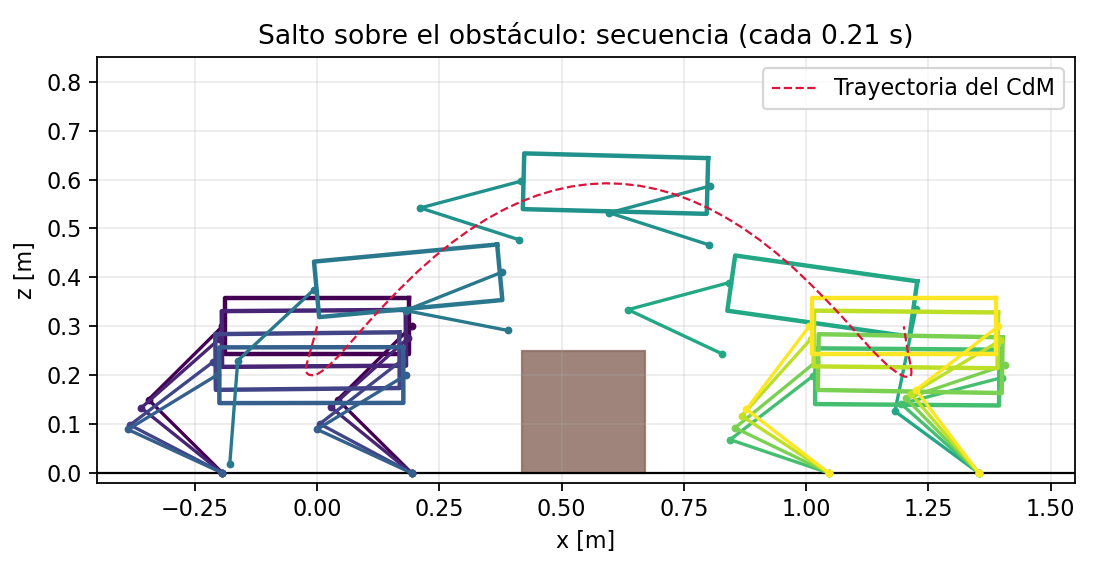
\includegraphics[width=0.5\linewidth]{p1_secuencia.png}
\caption{Secuencia del salto sobre el obstáculo.}
\label{fig:p1_sec}
\end{figure}

En vuelo alcanza una altura máxima del CdM de $\approx0.59$\,m, recoge las patas para librar la caja y aterriza primero con las delanteras y luego con las traseras, deteniéndose en $x_f=1.20$\,m tras una duración total cercana a $2.1$\,s. 

\begin{figure}[h]
\centering
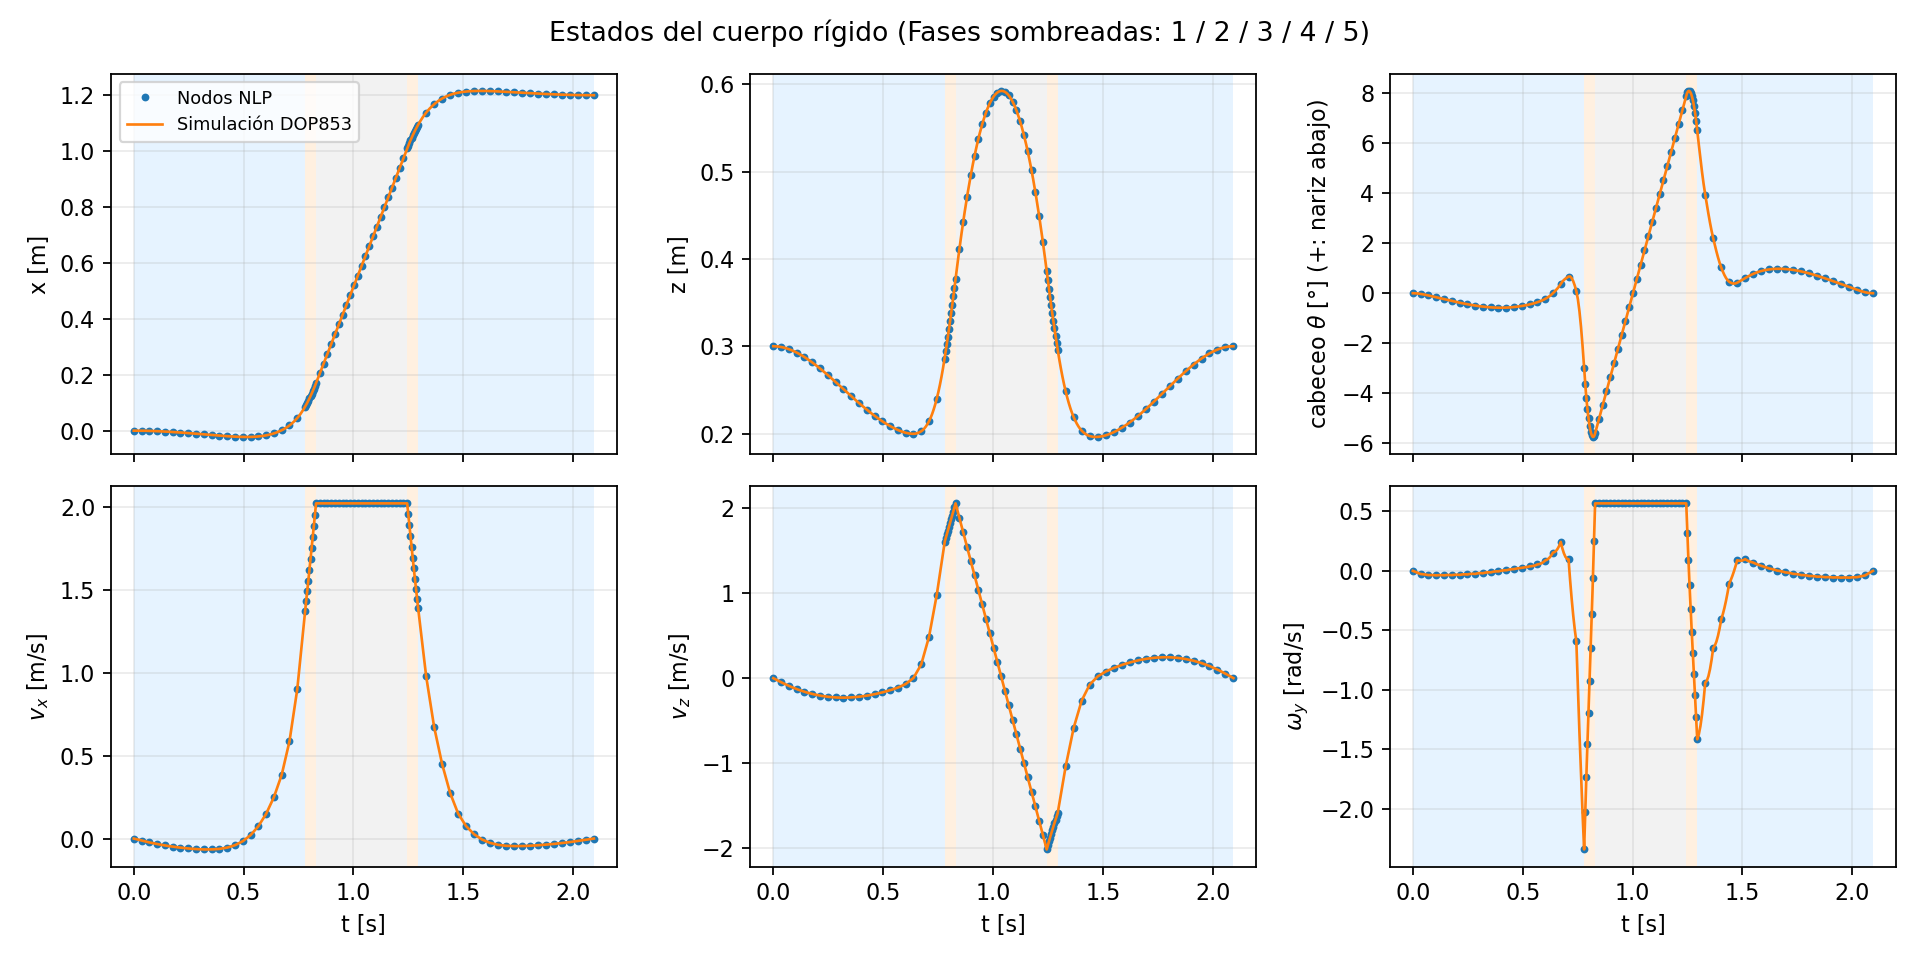
\includegraphics[width=0.5\linewidth]{p1_estados.png}
\caption{Estados del cuerpo rígido. Las bandas sombreadas indican las fases 1 a 5.}
\label{fig:p1_estados}
\end{figure}

\textbf{Animación.} Se adjuntan las animaciones \texttt{p1\_salto.gif} (velocidad normal) y \texttt{p1\_salto\_slow.gif} (cámara lenta).